\newpage

\section{Domain Classification}

\begin{figure}[h]
 \centering
 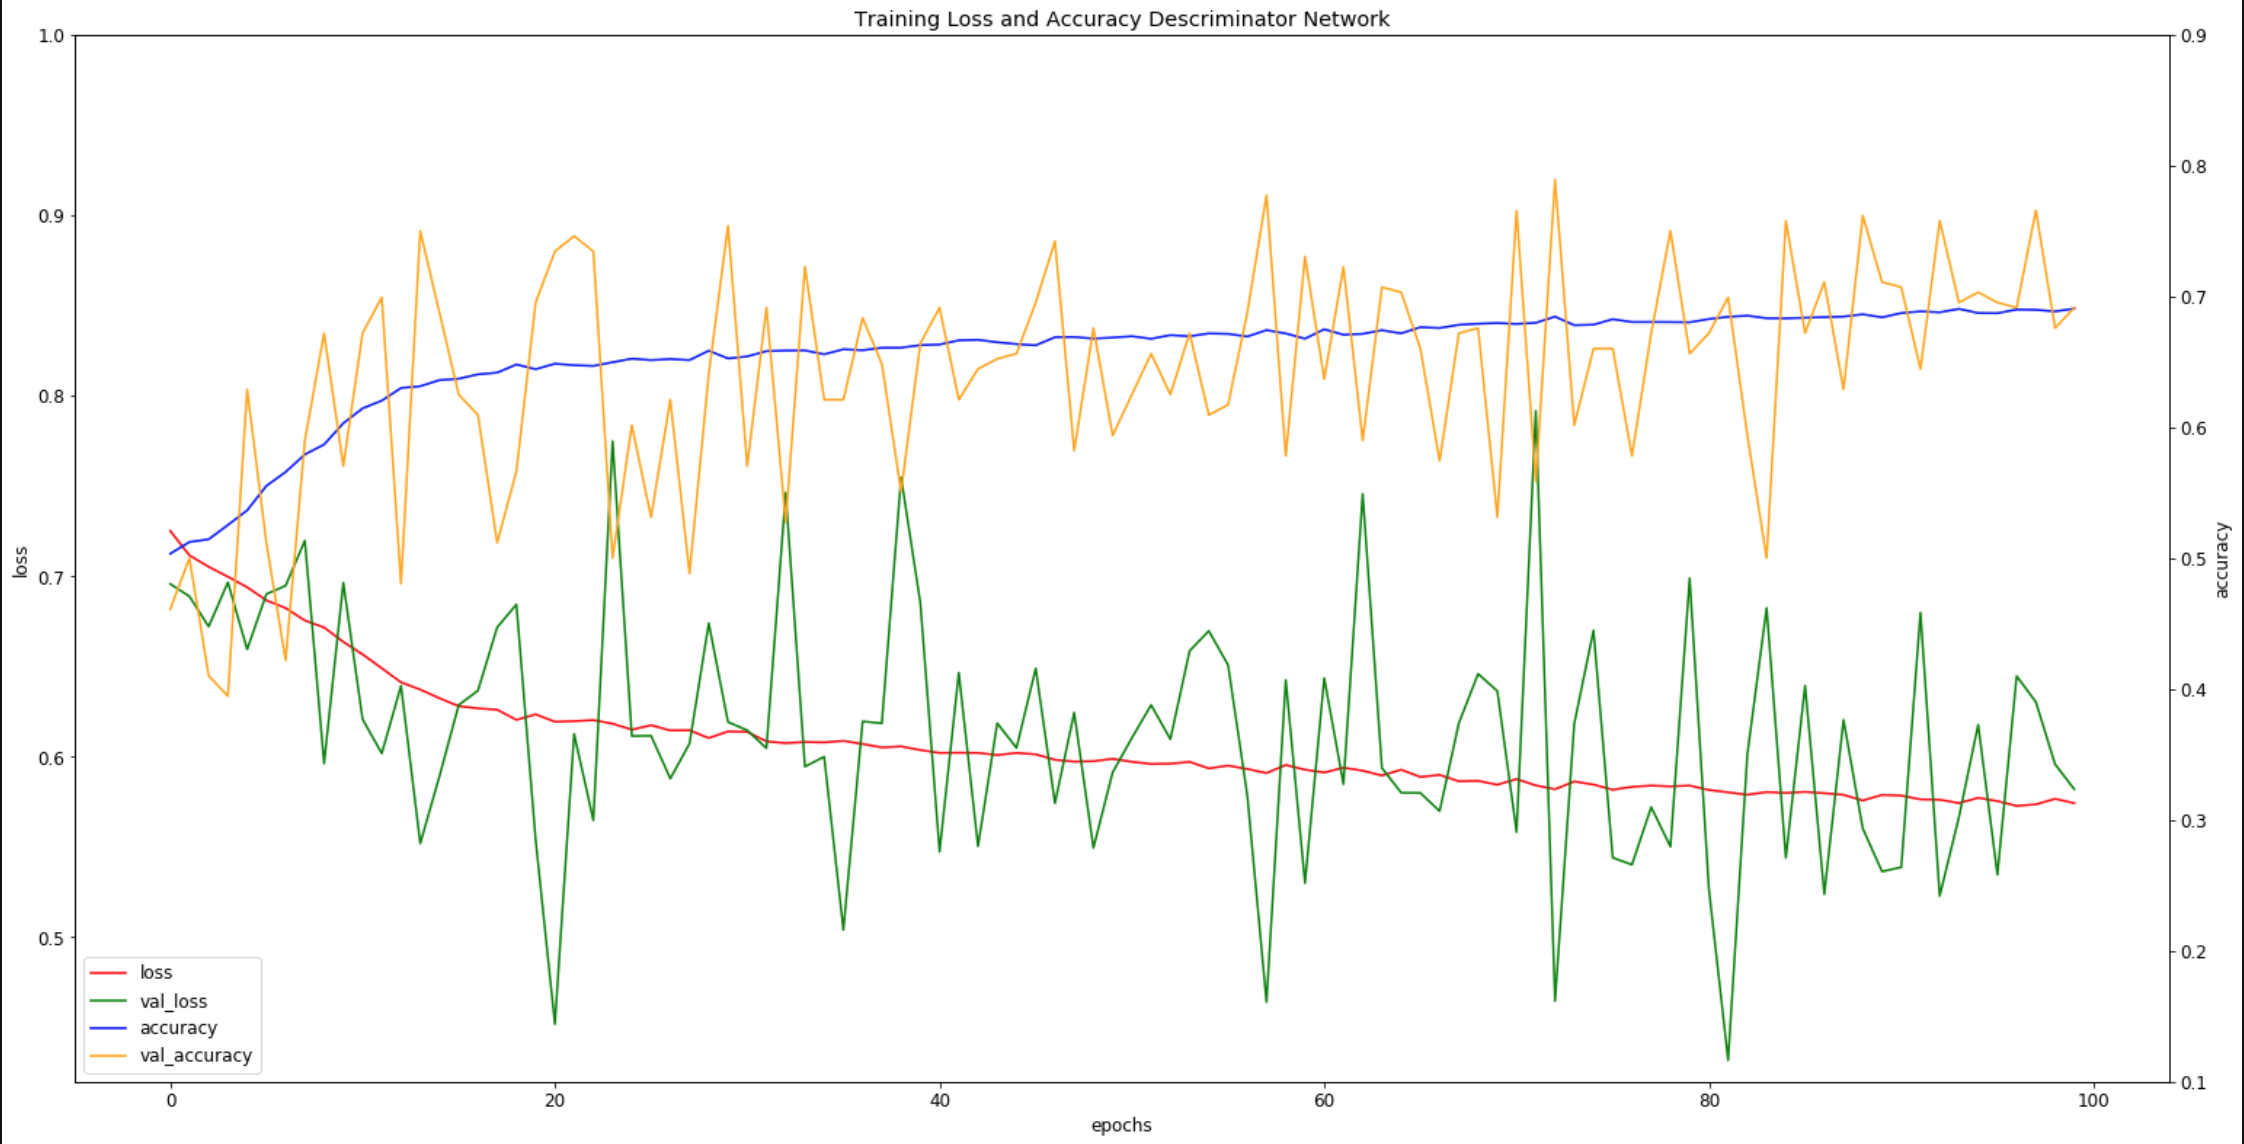
\includegraphics[width=160mm]{Descr/train.png}
 
  \textbf{Figure 34.} \textit{Network training and validation accuracy and loss for a discriminator network. The network was trained over 100 epochs using both GENIE and GENIE generated events. With an equal number of all three event types.}
\end{figure}

\begin{figure}[t!]
 \centering
 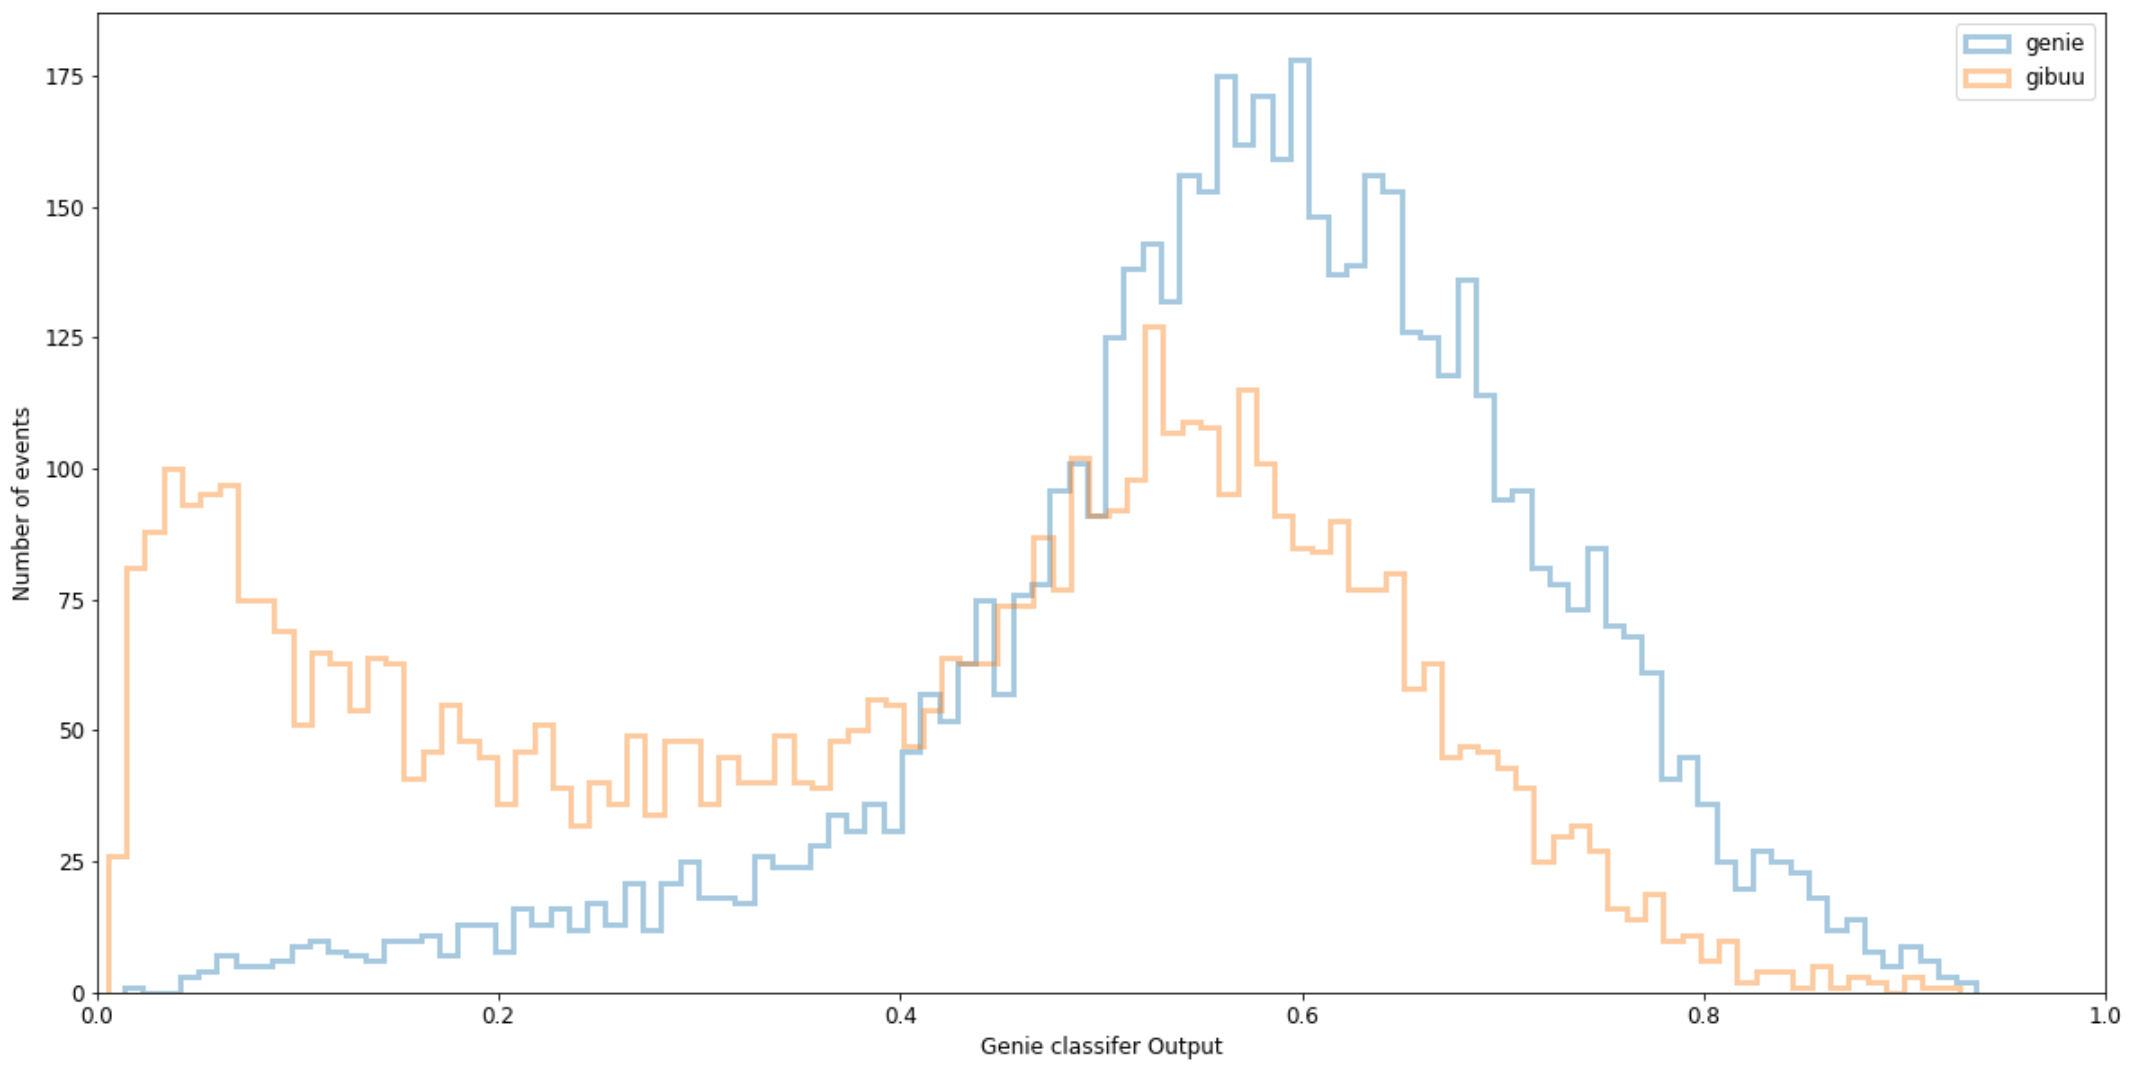
\includegraphics[width=160mm]{Descr/class.png}
 \textbf{Figure 35.} \textit{GENIE event classification output histogram. The dataset was trained and tested using an equal number of GENIE and GiBUU generated events. The dataset contained an equal number of the interaction types.}
\end{figure}

\begin{figure}[t!]
 \centering
 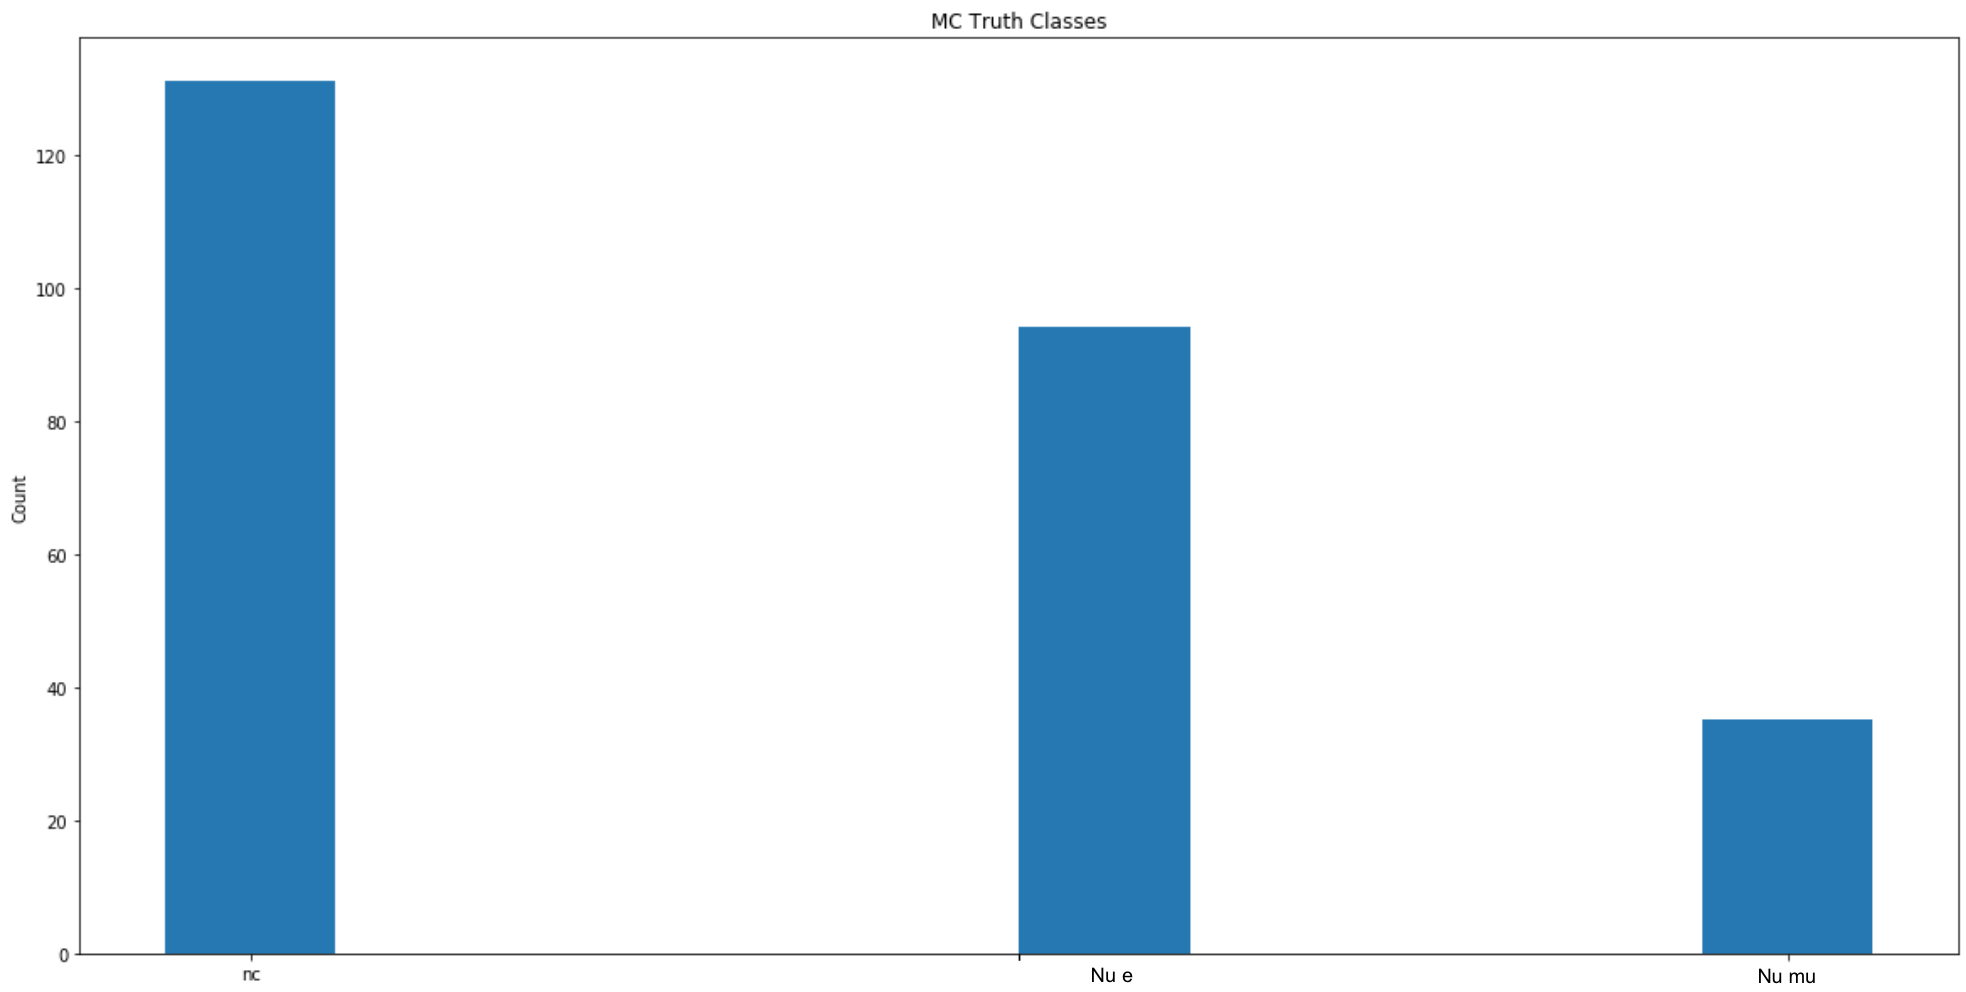
\includegraphics[width=160mm]{Descr/int.png}
 \textbf{Figure 36.} \textit{Histogram of the interaction types of events that the discriminator correctly identified as GiBUU events, with a confidence of greater tha 70\%}
\end{figure}


\noindent The network was modified to classify the events according to their production domain. In the training there were an equal number of GENIE and GiBUU events, as well as an equal number of each interaction type, to ensure that the model could train fairly and was not influenced by the distribution of events that may or may not be indicative of the domain. In Figure 34, the model does not appear to overfit, and the increase in accuracy tends to zero very quickly within the 100 epoch training process. The classification distribution can be seen in Figure 35 where there GENIE classifier output can be seen. The GiBUU classifier output is not shown as this is a binary classification task, and the GiBUU classifier is identical to that of the GENIE classifier simply reflected about the y-axis. \medskip

\noindent From Figure 35 we can see that the network struggles to classify the events from the two domains with confidence. Majority of the GENIE events are correctly classified with a probability between 50\% and 75\%. However with a very similar probability distribution a large proportion of the GiBUU events are incorrectly classified as GENIE events, indicating that these events are similar in appearance. However, with a confidence of 80\% and above (20\% and below on the GENIE classifier) the classifier correctly identifies a number of GibUU events, indicating that these events are fundamentally different in nature to the other GiBUU events, as well as the GENIE events that were incorrectly predicted as not GENIE events with a confidence of 80\%, and it is this difference in production nature that may cause bias in the interaction type classification when classifying events from the two different domains.\medskip

\noindent Figure 36 shows the interaction type of the events that are strongly classified as GiBUU events. There is a spread in the event types rather than one event type in particular being produced differently by GENIE and GiBUU. The $\nu_\mu$ feature the least here and one would expect this is because of the nature of $\nu_\mu$ interaction where the resultant $\mu$ leaves a very definite track. This may also explain why the classifier in section 3.1.4 was much more confident in correctly predicting the $\nu_\mu$ events- because they are easier to distinguish, as well as there being less variation between how the events are simulated between GENIE and GiBUU. \medskip

To try and understand the physical properties of these events, in Figure 37 the number of hits value is plotted for the GiBUU events that were classified as definitely GiBUU events, with a GENIE output value of less than 0.2, the GENIE events of the same GENIE output value and the GiBUU events with a GENIE classification output value of greater than 0.3. What can be seen is that the GiBUU events that were easily distinguishable are unique in their physical properties. They, on average, produce a much larger number of hits, than any other event, and in Figure 38 are seen to have much larger sum of FLS hits that made CellHits from this neutrino, energy values- unlike the rest of the events that typically have very low energy values here. The large number of hits suggests that these events have large showers- it then makes sense that they are mostly comprised of $\Nu_e$ events and $NC$ that look very similar.


\begin{figure}[t!]
 \centering
 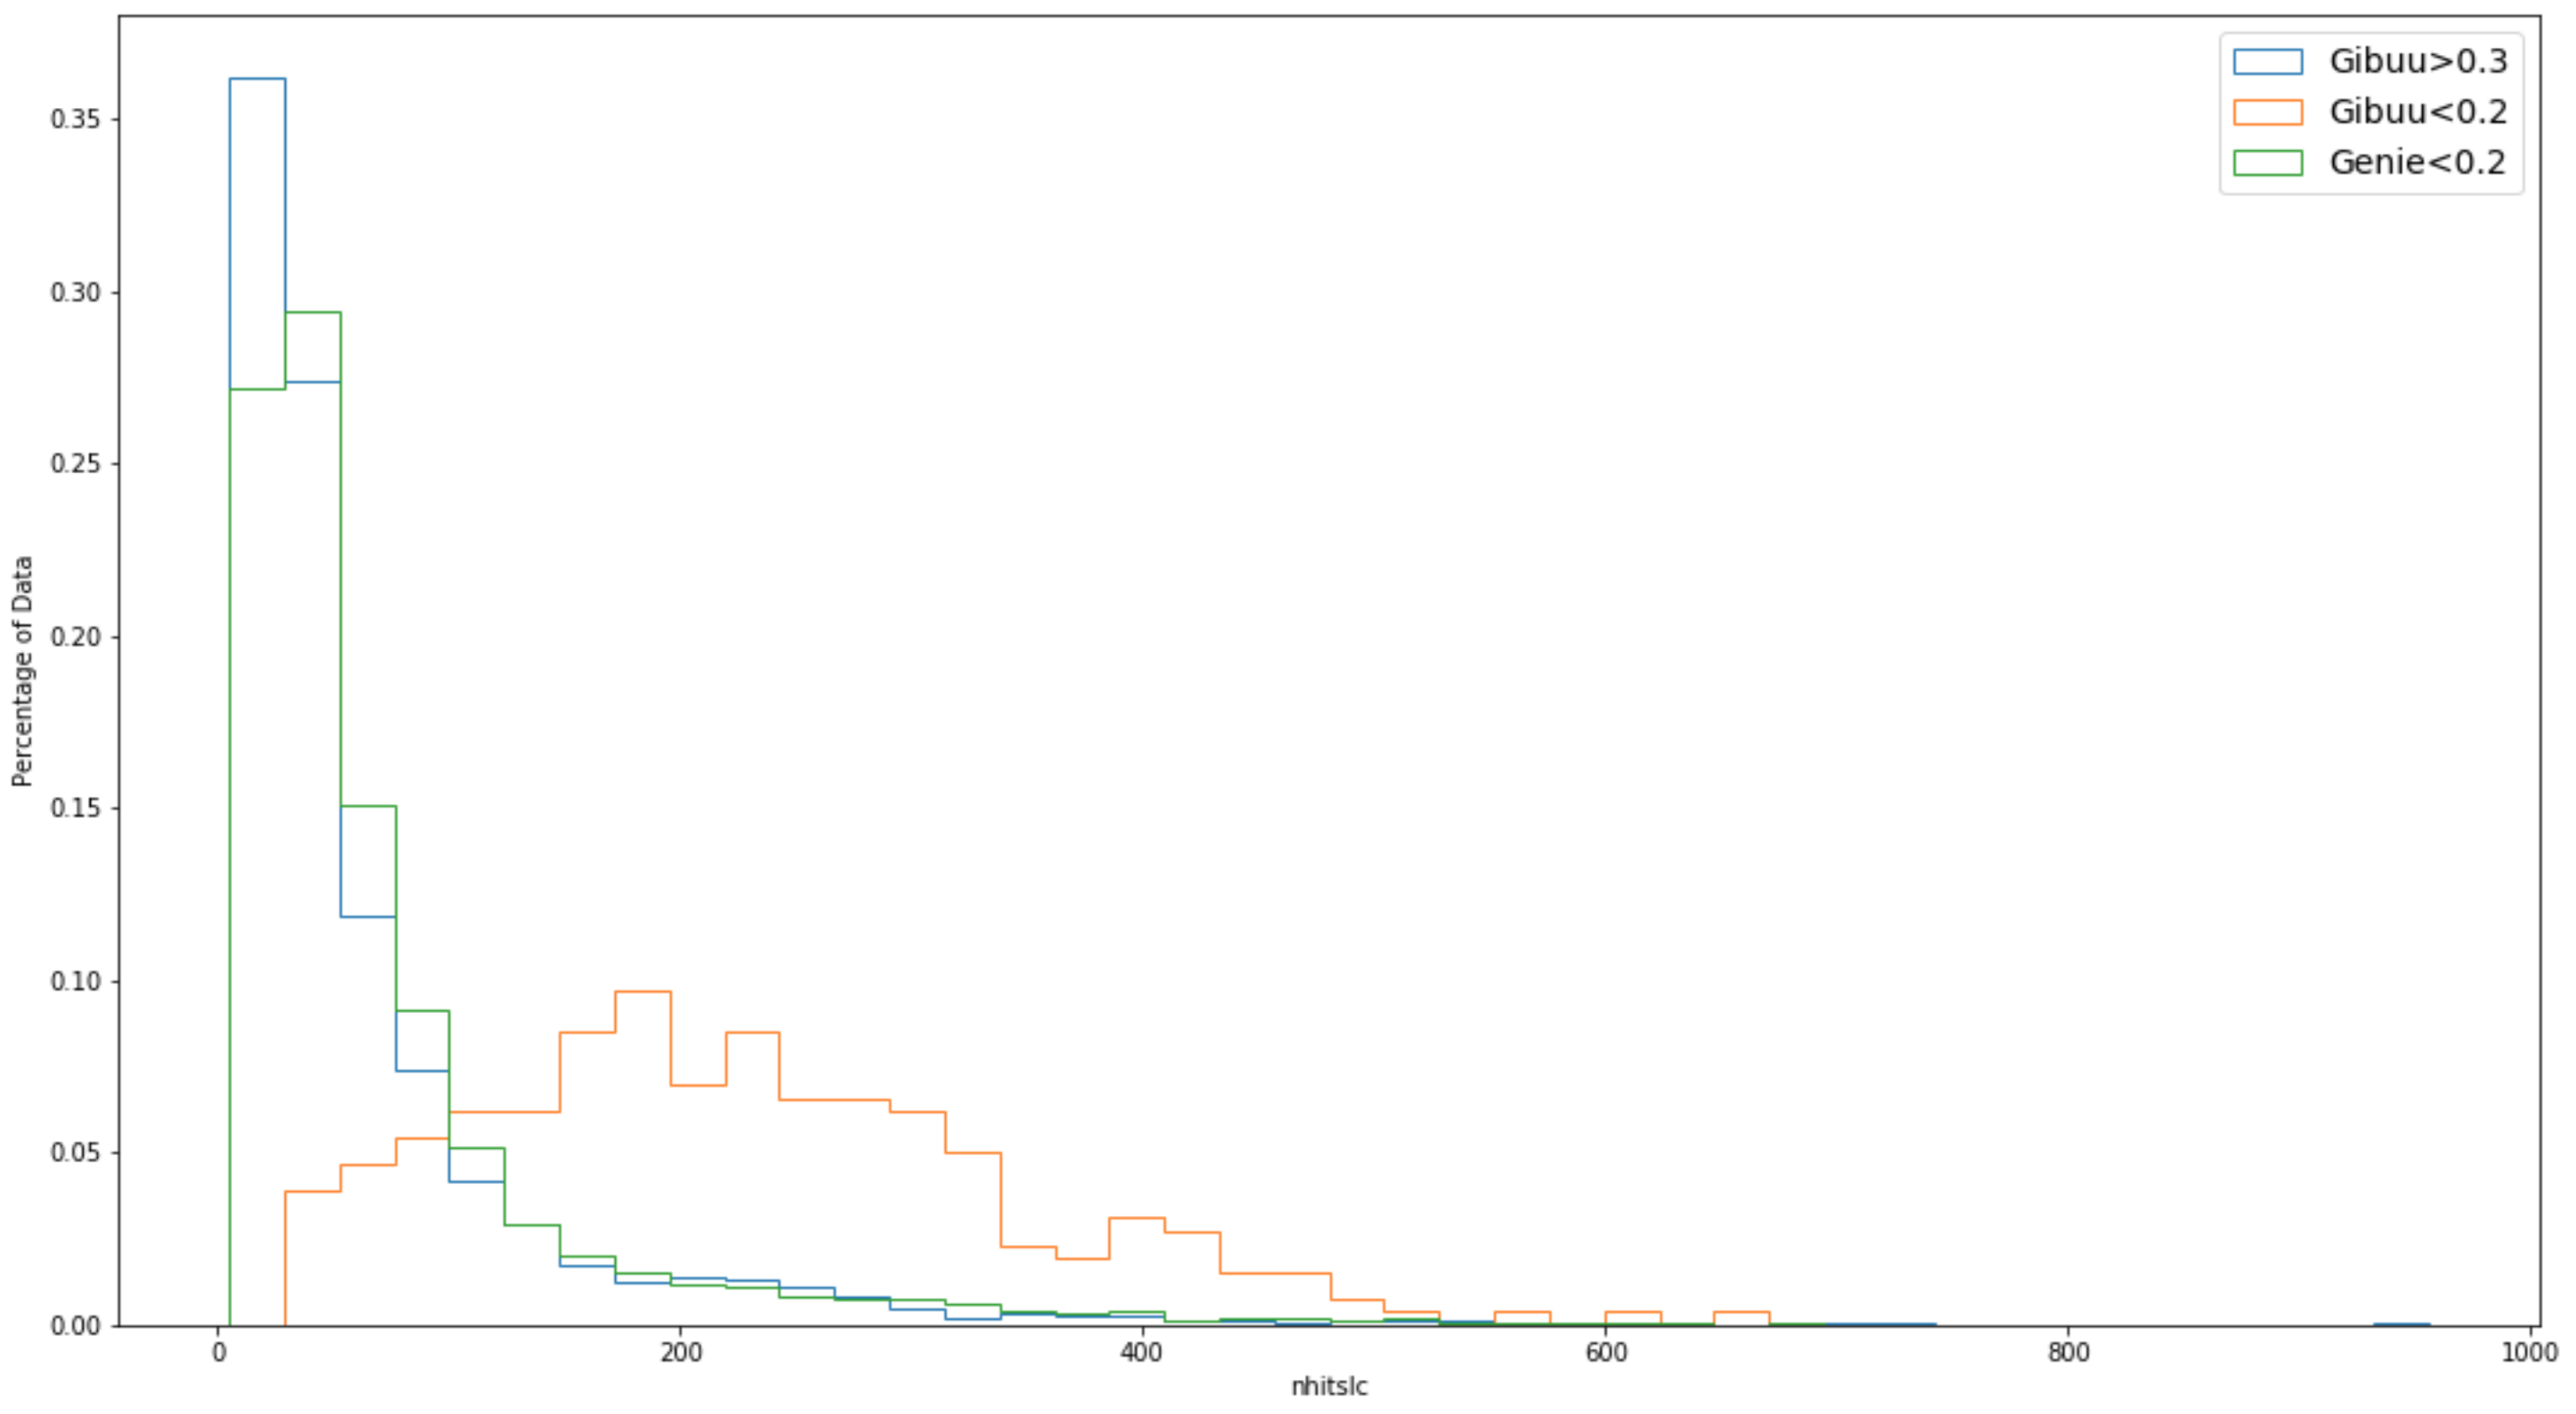
\includegraphics[width=160mm]{Descr/nhits.png}
 \textbf{Figure 37.} \textit{nhitslc- number of hits value plotted for events that with GENIE classification values of less that 20\% for both GENIE and GiBUU events, and greater than 30\% for GiBUU events, from the discriminator network}
\end{figure}

\begin{figure}[t!]
 \centering
 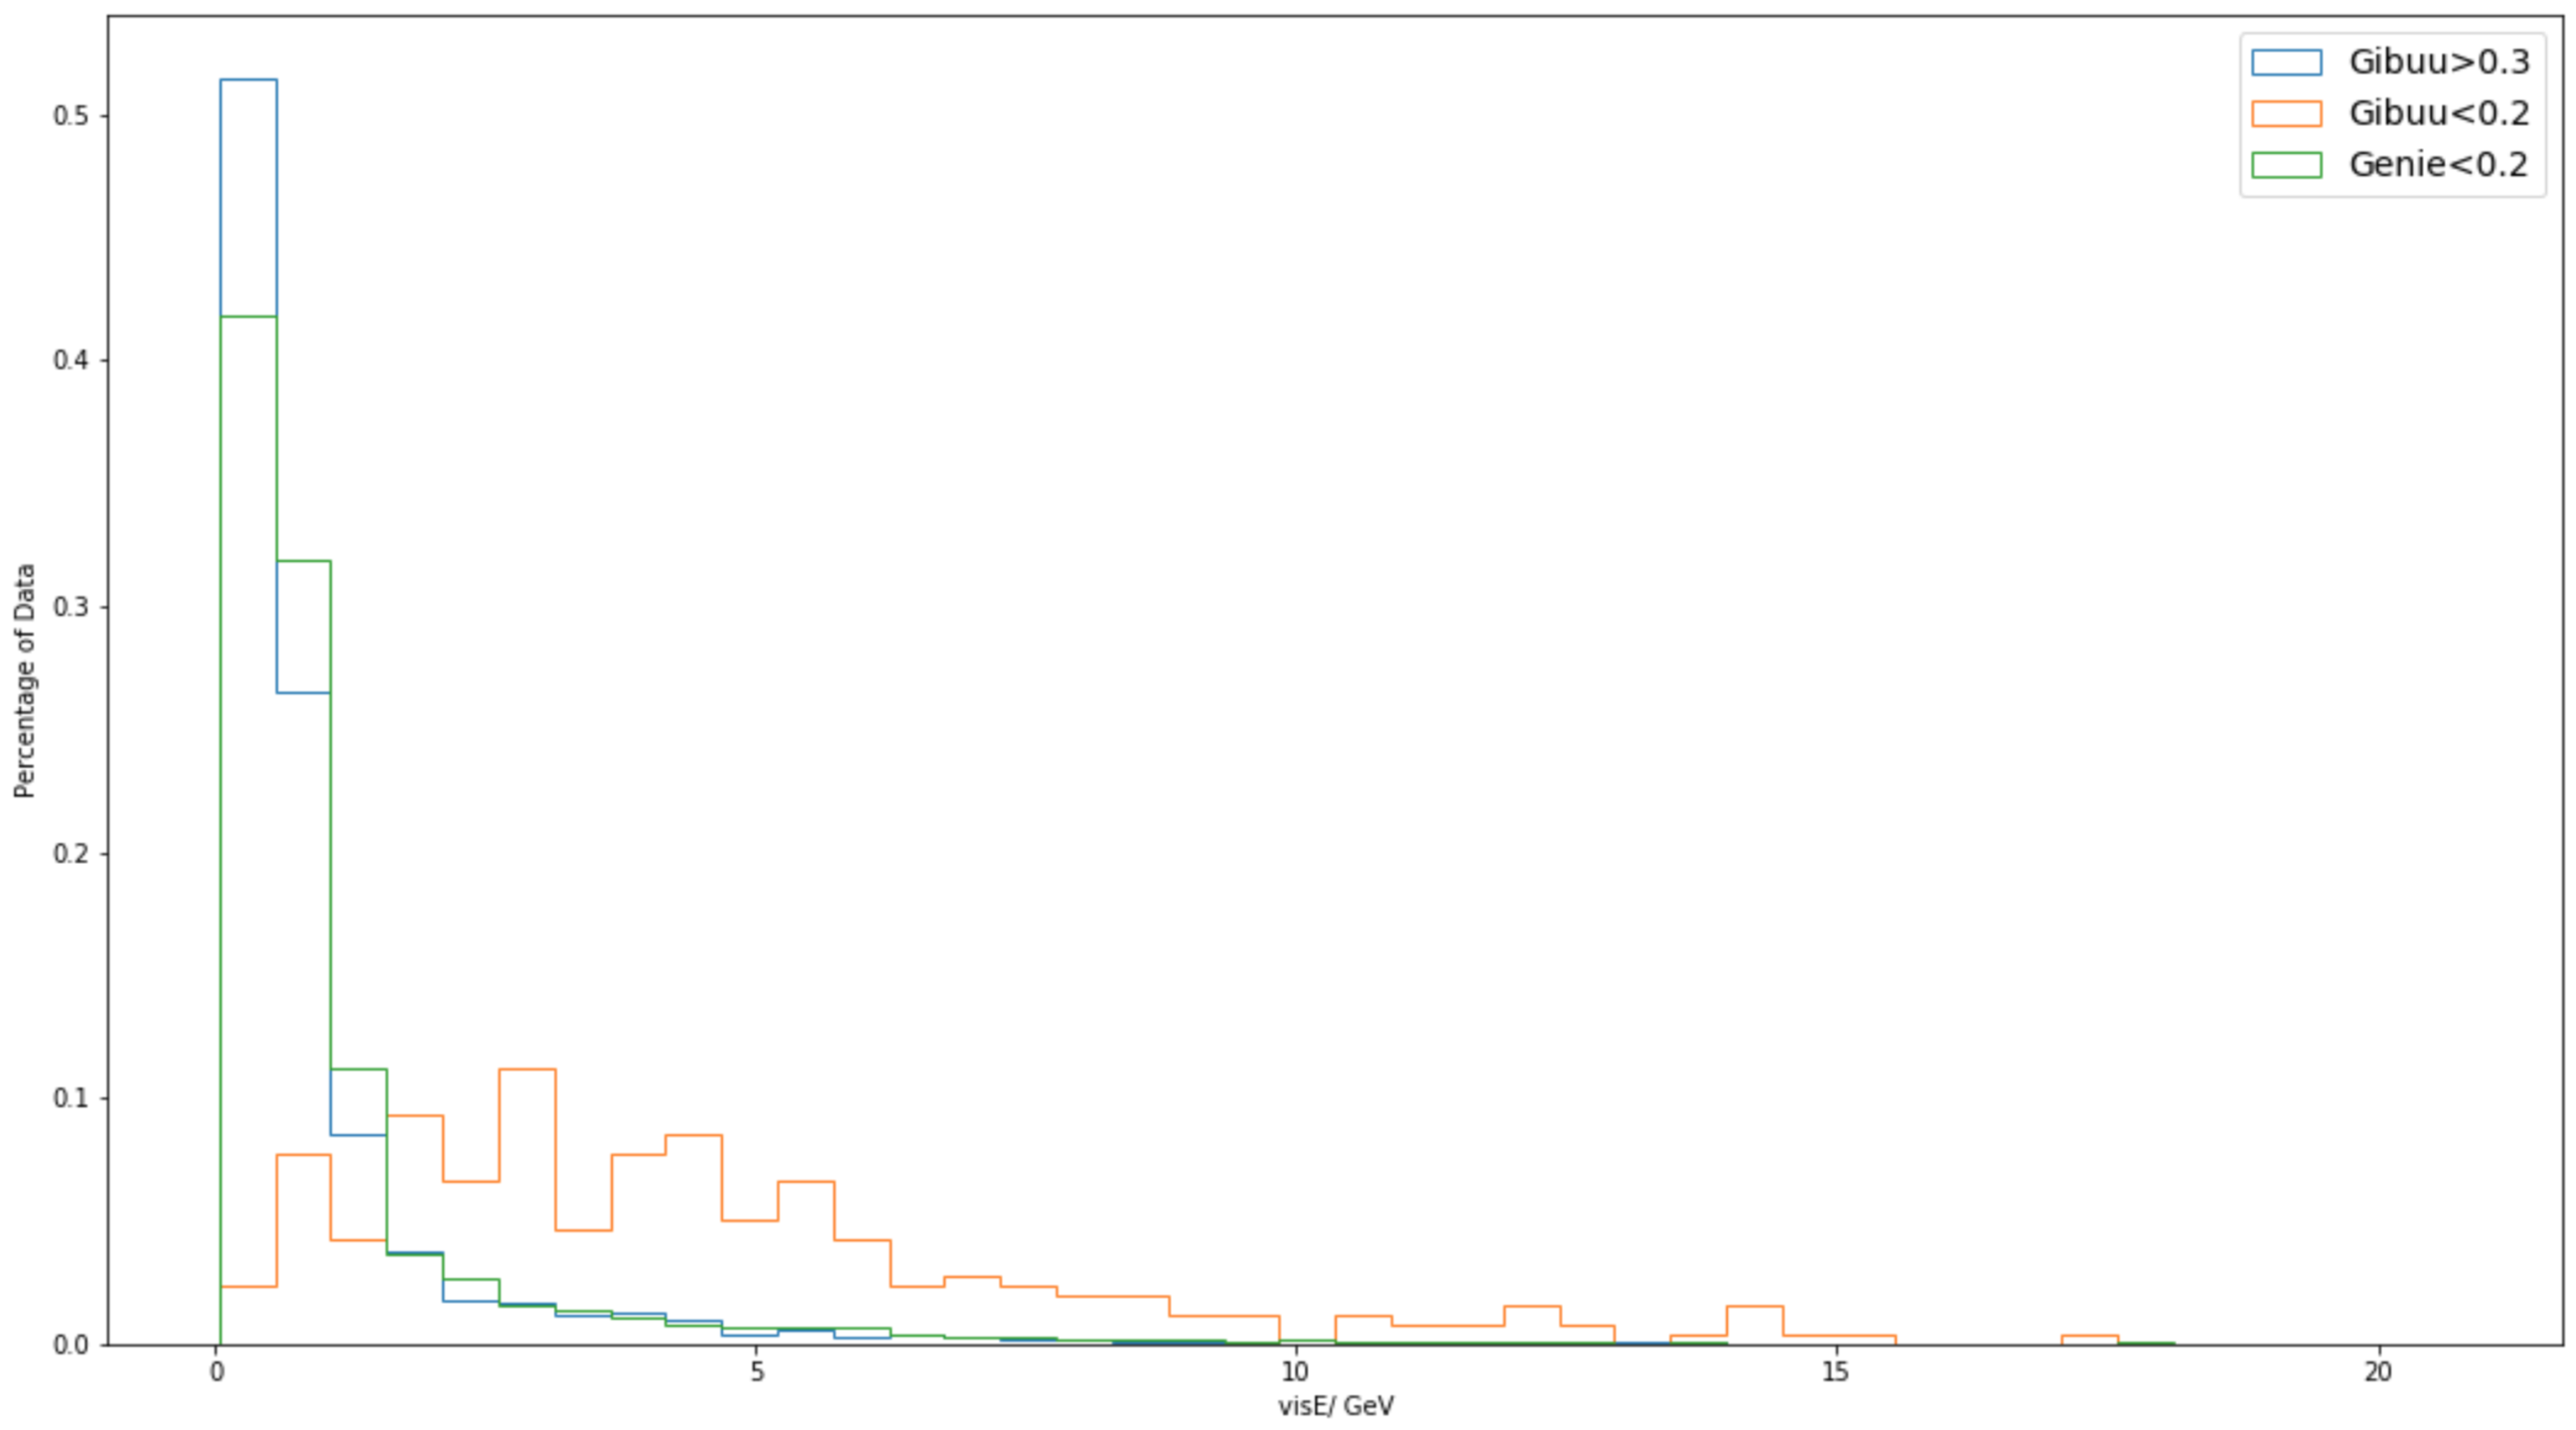
\includegraphics[width=160mm]{Descr/visE.png}
 \textbf{Figure 38.} \textit{visE- sum of FLS hits that made CellHits from this neutrino, energy value value plotted for events that with GENIE classification values of less that 20\% for both GENIE and GiBUU events, and greater than 30\% for GiBUU events, from the discriminator network}
\end{figure}

\newpage
